% !TEX root = main.tex
\chapter{Design and simulation of the addressing setup}
The purpose of this thesis work was to design and build the addressing setup for the already existing experiment. In this chapter we discuss the design and the implementation of such setup. The design is a crucial part of the work, there are several requirements that have to be met in order to achieve the proper needed functionality. In the first section, the requirements are presented together with an overview of the design idea. In the setup an objective was already present, and the choice of an AOD was already made. Hence, we discuss this components as given. The rest of the setup was simulated with the software Zemax, which was used to find the optimal optical components and their placement.
\section{Addressing system overview and requirements}
Addressing systems have already been developed and employed in experiments successfully. Different techniques are available: the main idea is to focus a laser beam tighter than ion-ion separation and steer it. In  Innsbruck calcium ions have been addressed in this way, where the steering was achieved with an AOD \cite{addressing}; Beam has also been steered with micro-electromechanical systems (MEMS) mirrors \cite{addressing3}. Another idea is to send a normal beam illuminating all the ions, but hiding those who are not addressed. This was done with Ytterbium atoms where by means of a inhomogeneous magnetic field the transition frequencies were shifted shielding selected ions \cite{addressing2}. \\
Our choice was to implement the already successful idea of Innsbruck with an AOD and improve it. The advantage of AODs is to have a fast switching time in the order of $\mu$s, that is used for fast switching between ions. A problem with the implementation of \cite{addressing} is however the fact that the AOD is placed right before the beam expander, this limits the addressing range, as the beam is likely to clip when it is steered on the edge of the AOD's bandwidth. This is the main problem that the new designed system, here implemented, wanted to address: exploiting the full capabilities of the AOD while maintaining a very tight focus.
Therefore, there are mainly two aspects to keep in mind, the focus spot and the addressing range. However the priority was the focus spot as a large addressing range is not essential.
\begin{figure}[H]
\centering
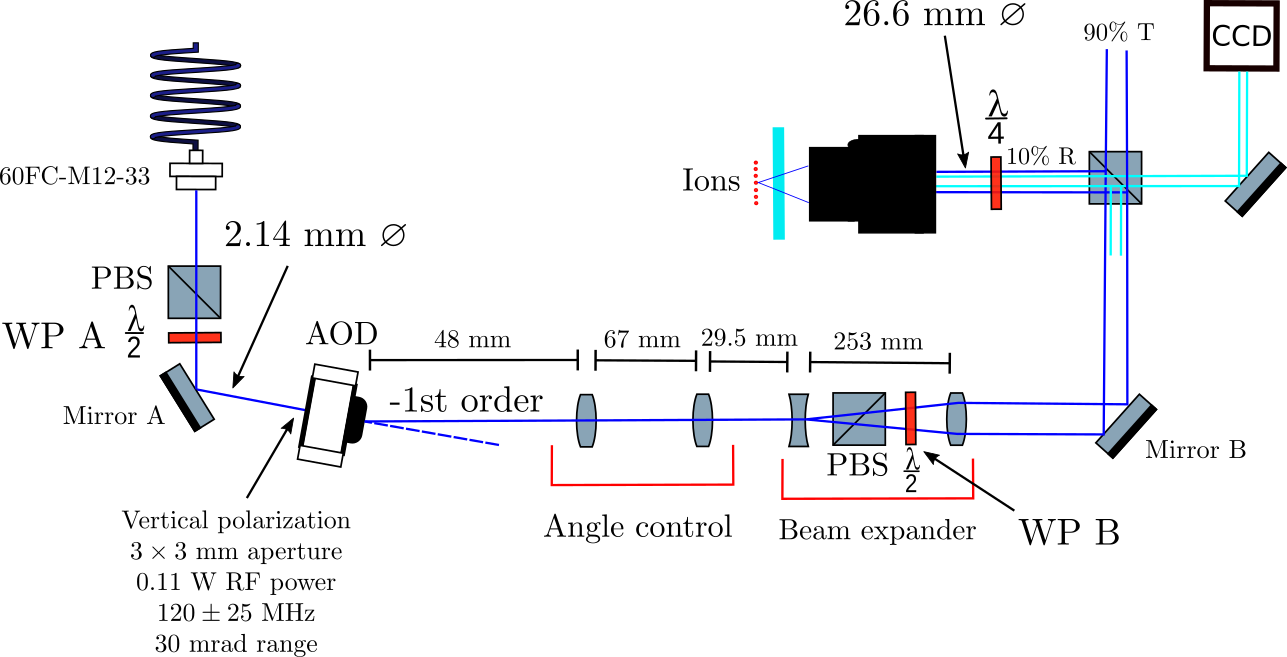
\includegraphics[width=\textwidth]{img/setup}
\caption{Scheme of the setup. Light comes from a fiber, polarization is cleaned, and then sent thorough the AOD. 1st order diffracted light is refocused into a beam expander, where the beam is broadened before being focus by the objective. Light blue lines represents 393 nm light coming from the ions into the imaging setup.}
\label{addressingsetup}
\end{figure}
The addressing setup should be able to address single ions in a string in order to generate single photons out of single ions via the already discussed Raman process. Ion separations, in the case of $^{40}\text{Ca}^+$, has been derived in section \ref{ionstrings}, for a trap frequency of 1 MHz is 5.6 $\mu$m. The setup must therefore be able to focus tightly a laser beam down to 1-2 $\mu$m. As seen in section \ref{sec_diffraction}, a tighter focus can obtained with a shorter wavelength, a bigger lens, or with shorter focal length. The focusing lens, a.k.a the objective, is shared with the imaging setup, and thus it is given, the focal length is therefore a constant in the problem. The wavelength is also a constant, as the Raman process happens only at 393 nm. This gives only one possibility left to tighten the focus, i.e. by making the beam as broad as possible at the objective input surface. Beam expansion can be achieved with a Galilean telescope, it take two lenses to form such Telescope, a concave Lenses to diverge a collimated beam and a convex lens to collimate the diverging beam. The combinations of these two lenses takes a collimated beam and expands it to another collimated beam. This expansion part is one of the two essential part of the addressing setup. The other part is related to addressing range. Not only, we want to focus the beam to a single ion, but we want to move the beam as well, such that it focuses on a different ion. Therefore, there is a requirement also on the range that can be addressed. This depends on the number of ions and their spacing, a good aim is to address tens of ions, this requires the ability to move the focus in one direction by 150-200 $\mu$m. Beam steering is possible with the use of an AOD, the detailed working principle of this device has been discussed in section \ref{theory_AOD}. Basically the angle of the output beam of the AOD changes as the driving frequency changes. However, the AOD must be placed far behind the objective to leave space for the beam expander, this implies a need to control and redirect the angle of the AOD's output beam to send it to the beam expander and later in the objective without any clipping. This task is accomplished with a pair of converging lenses, they refocus the collimated beam into the beam expander, beam then becomes wider, reaches the objective and it is focused on the ion. It is important to get the right lenses at the right distances, the objective has 5 different lenses inside and it works slightly differently from a normal lens. For instance, it does not focuses collimated blue light, but red. This means that the beam expander should not collimate completely the beam but rather expand it and leave it diverging, so that the objective can focus it at the right position.
The setup displayed in figure \ref{addressingsetup} also contains polarization optics. As discussed in section \ref{sec:ramanprocess}, Zeeman transitions are polarization sensitive, thus polarization control is required. The AOD is polarization sensitive, which means it requires a certain input polarization and outputs another particular polarization, that is the reason why half wave plate are before and after, and additional quarter wave plate is inserted before the objective to obtain circular polarized light. This placements means having a non standard plate, but if placed before in the optical path, the mirror and the beam splitter could alter the polarization. The choice of using a beam splitter is also peculiar, to separate light at different wavelength it is common choice to use a dichroic mirror, however the light in the imaging path is 397 nm, very close to the 393 nm light of the addressing setup. This would have meant using a very narrow dichroic, the alternative was to use a 90:10 beam splitter, where 90 \% of the light is transmitted and only 10 \%of the light is reflected. The addressing therefore loses 90 \% of the power on this splitter, but that is not a problem, since it is always possible to get more light out of the laser. Furthermore, this light is focused so tightly that even a small amount of light can excite the ions. On the other end, it is not really possible to get more scattered light from the ions, so 397 nm light and the imaging setup must be as efficient as possible, with 10 \% of losses, ions are still visible on the camera and on the PMT.


\section{Objective and AOD}
\label{sec:obj}
\begin{figure}[H]
     \centering
     \begin{subfigure}[b]{0.4\textwidth}
         \centering
         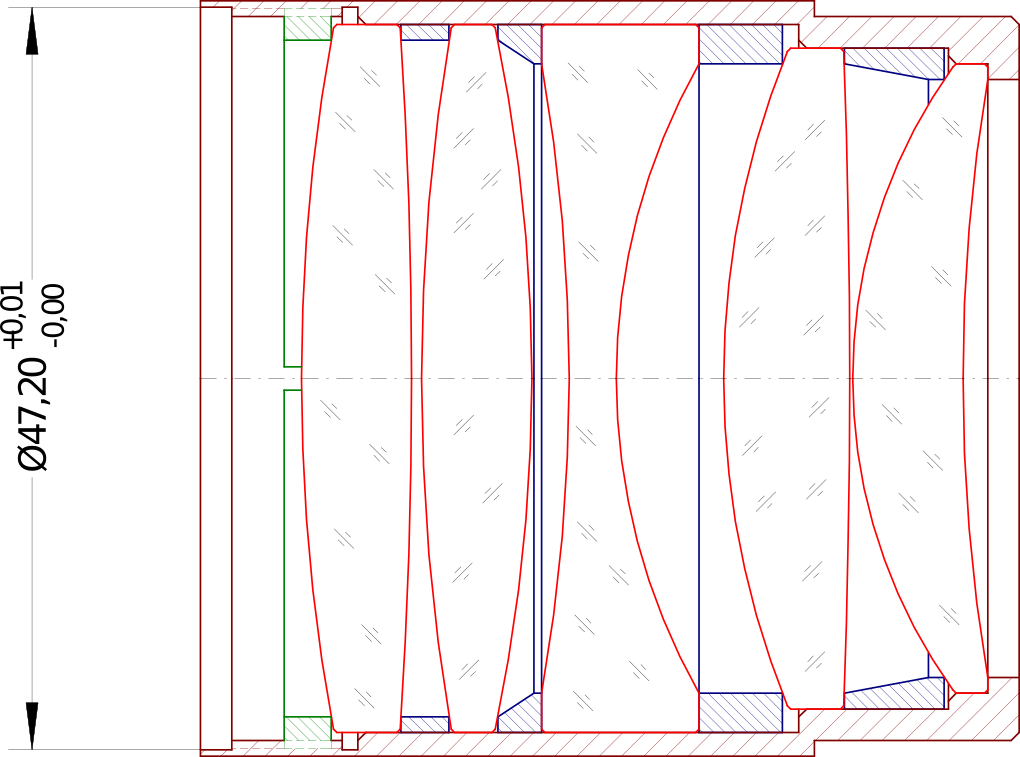
\includegraphics[width = \textwidth]{obj}
          \caption{Section of the custom objective, red parts are the lenses, while the rest is the housing.}
         \label{objsection}
     \end{subfigure}
     \hfill
     \begin{subfigure}[b]{0.55\textwidth}
         \centering
         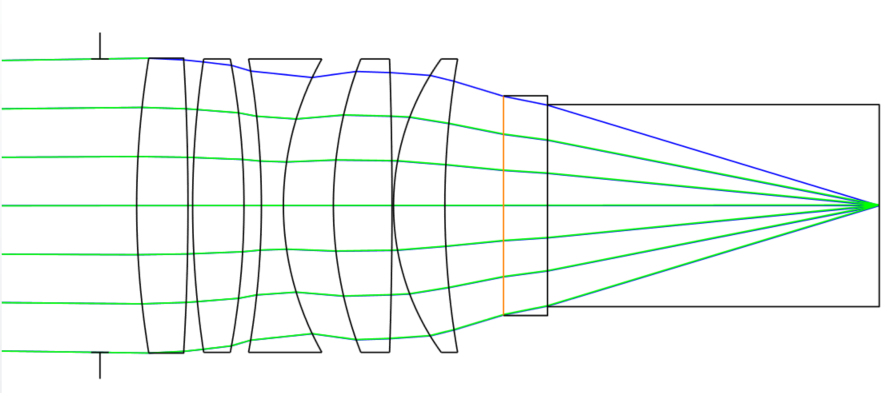
\includegraphics[width=\textwidth]{zeemaxobj}
         \vspace{1em}
         \caption{Zemax simulation of the objective. On the right, viewport and the vacuum chamber are also present.}
         %\label{fig:three sin x}

     \end{subfigure}
        \caption{}
      %  \label{fig:three graphs}
\end{figure}
The objective used to focus the light was already present in the system and had to be taken as it is. It is a custom objective by Sill optics placed outside vacuum, the section is in figure \ref{objsection}. It contains 5 lenses inside a mechanical housing, the aperture is about 47 mm large in diameter.
This objective has different purposes, it was designed keeping in mind: imaging of ions, addressing with red light and addressing of blue light. The objective has to perform all three of this jobs fairly well, which means it has light transmission >90 \%, every lenses is AR coated, numerical aperture of NA = 0.3. Moreover, it is telecentric, which means that the focus spot should move perpendicularly to the optical axis if the beam is steered.
 Lastly it was also designed to take into consideration the fact that it is placed out of vacuum, the light after the objective has to go through a 6 mm fused silica viewport before entering the vacuum and after further 40 mm encounters the ions. The focal length of the objective is 54.07 mm at 729nm. The objective is also mounted on a 3 dimensional translational stage to allow for imaging and addressing calibration.\\
The AOD is from Gooch \& Housego, model 4120-3. It has a specified central frequency of 120 MHz, with 50 MHz, bandwidth, so the driving frequency ranges from 95 to 145 MHz with a maximum RF power of 0.3 W. Therefore, the angle of deflection should be $\pm 0.86^{\circ}$ (:|).  In this bandwidth the diffraction efficiency should remain above 75 \% and have an average of 83 \%. Further light is lost as much as 3\% of due to insertion losses. The active aperture measures $3\times 3$ mm, and the polarization has to be horizontal when entering the AOD, while it gets rotated during diffraction, as the specified output polarization is vertical.

\section{Design simulation}
The setup in figure \ref{addressingsetup} has been simulated with the software Zemax. The simulation had the purpose of assessing the performance of the setup, i.e. checking the viability of the setup and see if it meets all requirements. It was also used to find the best lenses for building the setup and the best placement. Not everything was simulated, bu only the essential parts. This includes the four lenses, the objective, the viewport and the vacuum chamber. As there is no option to simulate an AOD, it was not taken in consideration, instead the simulation started at the output of the AOD as described below. Mirrors and beam splitters also do not alter drastically the optical path and therefore there was no need to simulate them.
\begin{figure}[H]
\centering
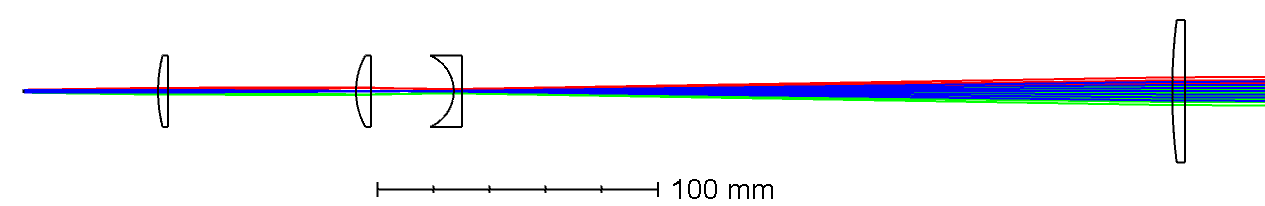
\includegraphics[width = \textwidth]{zemax3d}
\caption{Zemax simulation of the setup. Rays propagate from left to right, only the four lenses are displayed, objective and image plane are far on the right. Different colors indicate different fields at different angle}
\label{zemaxview}
\end{figure}
The simulations start by specifying the input fields, these represent the physical light beam. To account for the different angled beams at the output of the AOD, three different fields has been simulated. One is along the optical axis, while the other two are angled corresponding to the extrema of the AOD bandwidth, so $\pm0.86^{\circ}$. Therefore the propagation of these beams represents three different situations of beam direction and should also give an idea of the behaviour in between the extrema. Next, the four lenses of the setup were inserted in Zemax, initially with variable radius and thickness. The Zemax file of the objective came from the company which designed it and was simply imported in the project. After the objective the 6mm viewport glass was included and then vaccum for 38.6 mm, which is the distance between the outer facet of the glass and the ion axis. The image plane was therefore set here. The distance between the last lens of the objective and the viewport was unknown, but a good estimation\footnote{A posteriori, this assumption was not well suited and lead to some errors in the test setup. The correct value could be found by simulating the imaging setup and optimizing this distance to get the focus onto the camera.} allowed to progress with the simulation.
They physical simulation in the software was carried out with the tool Physical Optics Propagation (POP). POP works by propagating a wavefront represented by an array of discrete points. The array is propagated through every optical component and free space. This method can be used to simulate coherent Gaussian beam with high precision as well as wave phenomena such as diffraction and aberrations. The initial value given to the propagator was the waist of the collimated beam out of the AOD. Since the beam going to the AOD comes from a fiber collimator, the value specified was taken from the datasheet of the fiber collimator, namely Sc\"after + Kirchhoff 60FC-M8-33 \cite{fibercollimator}. Therefore, the specified waist was 0.72 mm.
\begin{figure}
     \centering
     \centering
     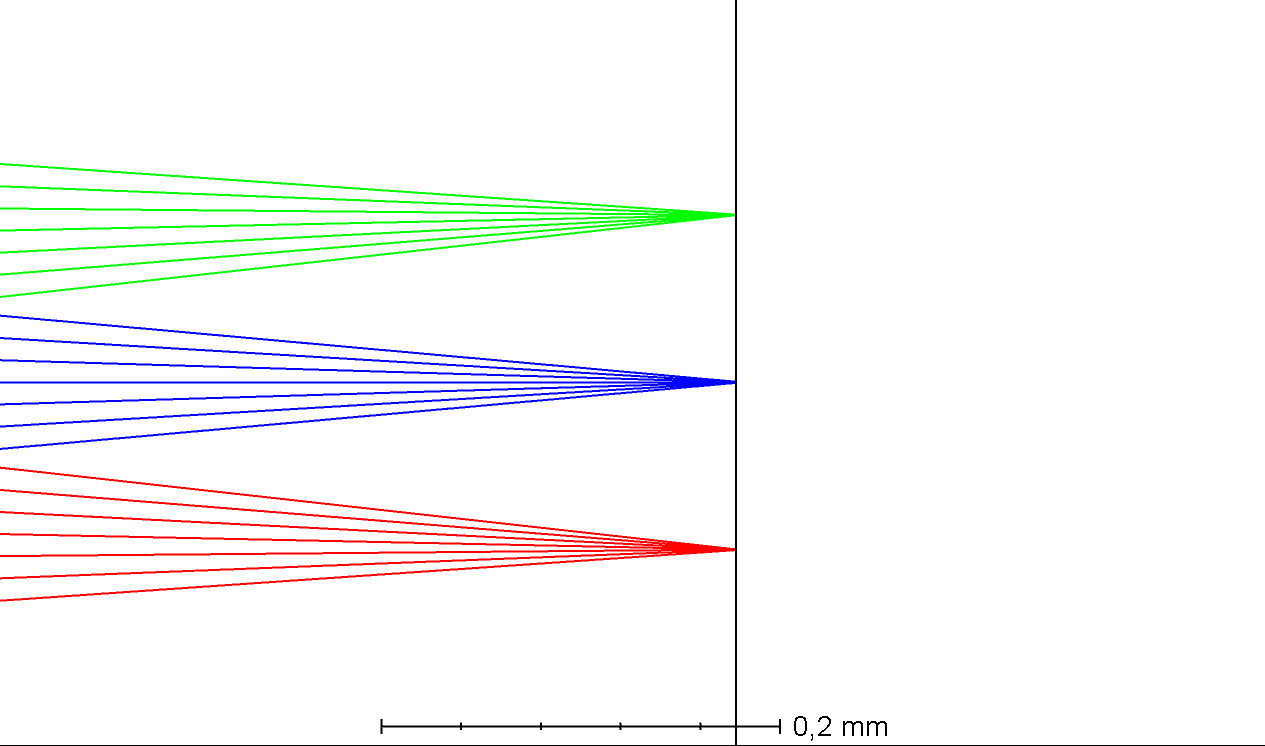
\includegraphics[width=.8\textwidth]{img/zemaxrange}
     \caption{Zemax simulation at the image plane, where the ions are. The three colors are three different fields with different angles that are focues at different position along the ion string. The full addressing range here displayed is about 168 $\mu$m.}
     \label{zemaxrange}
\end{figure}

\begin{figure}
    \centering
    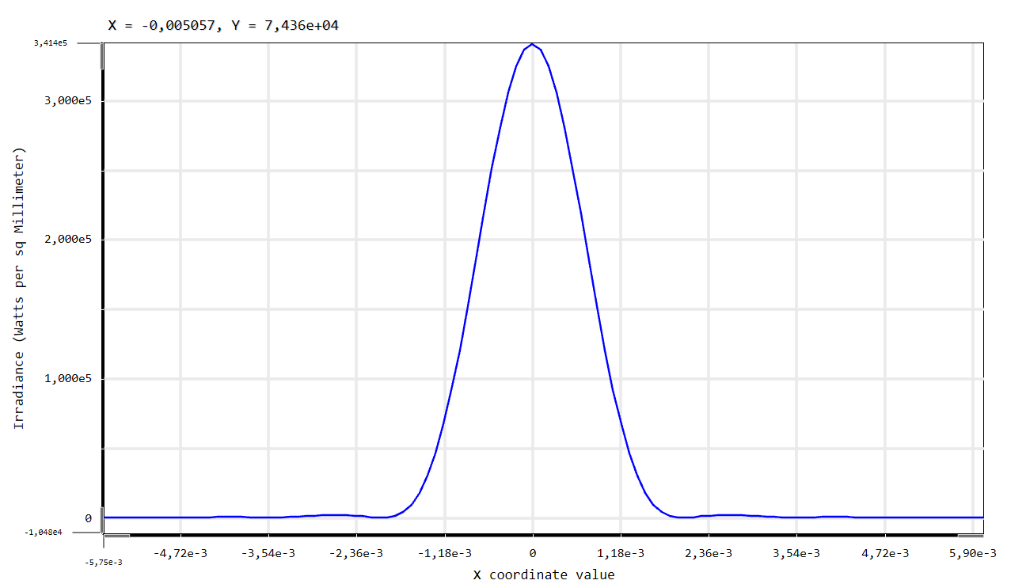
\includegraphics[width=.8\textwidth]{img/zemaxfocus}
\caption{POP of the central field at the ion position, $x$ cross section is displayed.}
\label{zemaxfocus}
\end{figure}
The first step of the simulation work was to find the appropriate lens to build the setup. The thickness and the radius of the lenses was optimized trying to achieve the best focus spot while maintaining a good addressing range. Once obtained the desired situation, the lenses were found with the Zemax tool \emph{Stock Lens Matching}. Basically the tool compares the simulated lenses with those in a catalogue from different companies and find the closest match. We opted to rely on the provider Thorlabs, so the search was limited to this company. Found lenses were in order from left to right LA-1059, LA-1131, LA-4252, and LA-1725 and can be seen in figure \ref{zemaxview}. Once the desired lenses were found, their Zemax files provided by the company were imported in the project and further optimization was carried on.\\
The second step was to optimize the lenses position always in view of finding the best focus spot while keeping a good addressing range. This was done using the optimiing tools of Zemax and the merit function. The software can perform multivariate analysis and minimize the focus spot depending on all the assigned variables, which in this case were the distance between the lenses. The final results can be seen in figure (), the addressing range is 168 $\mu$m, while the waist is $1.3\,\mu$m.\\
 Another important parameter for the performance of the setup is the addressing error. In the case of the beam focused on one ion, the addressing error is the leaking light on the neighbours ions. It can be a problem in the case of aberrations that produce bumps on the side of the main Gaussian peak. Especially in the case of diffraction limited system, the profile of the beam is a sinc function that can have more local maxima around the central peak. To estimate the addressing error, two ions are placed next to each other at 5.6 $\mu$m, and the respective addressing beam has been simulated. The intensity profile has been plotted in figure \ref{zemaxaddrerror.png} and addressing error is calculated as $I_1(x_2)/I_1(x_1)$, where $I_1$ is the intensity profile of the beam focused on the left ion and $x_1,x_2$ are the positions of the two ions. From the simulations we get $I_1(x_2)/I_1(x_1) \simeq 9 \times 10^{-4}$.\\
 \begin{figure}
 \centering
 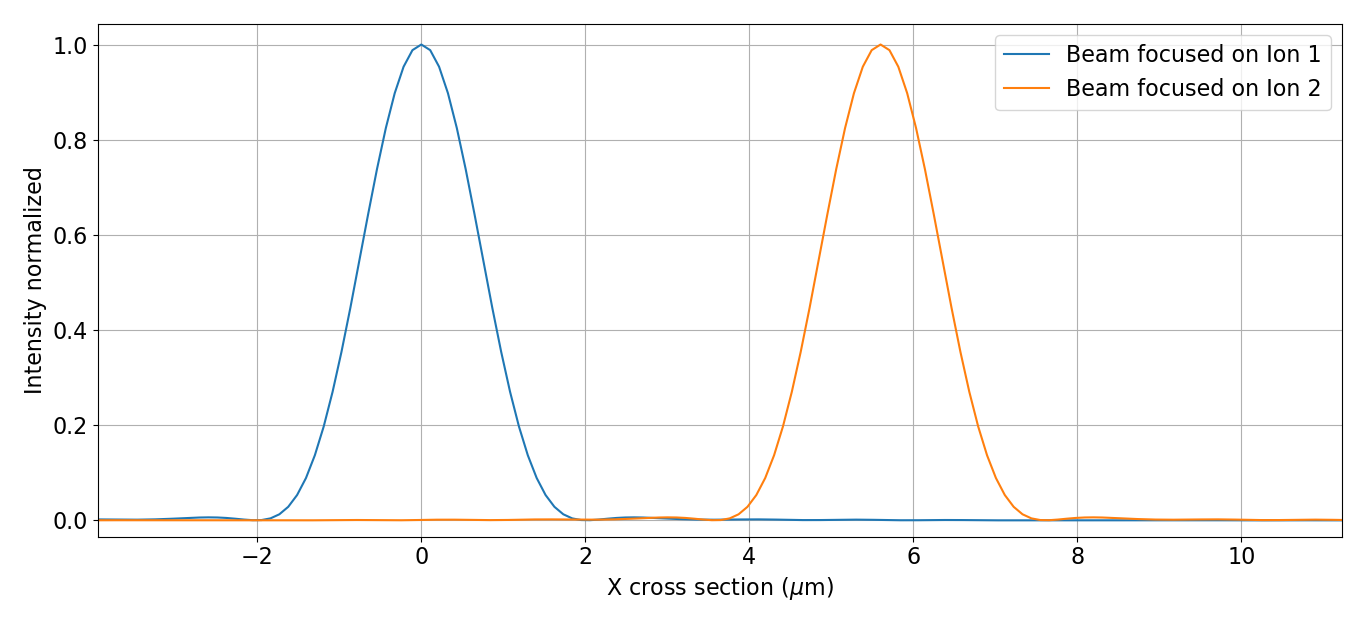
\includegraphics[width = .9\textwidth]{zemaxaddrerror.png}
 \caption{Beam focused at two different positions, where ions have their equilibrium position. From estimation of the addressing error can be made.}
 \label{zemaxaddrerror.png}
 \end{figure}
Another aspect that was simulated is the beam profile inside the trap. Optical access to the trap is limited and a tightly focus beam also has a large divergence, which could lead to clipping on the trap's blades or compensation electrodes scattering light all around the trap and thus creating problems. In figure \ref{clippingtop} the top view of the trap is plotted. The blue line represents the radius $W(z)$ from equation \ref{waistprofile} of the addressing beam in the case of a waist $W_0$ of 1 $\mu$m. There is no apparent clipping, and the main problem seems to be the compensations electrodes. Since the the beam is Gaussian, there is always a clipping part. To determine the fraction of power lost due to clipping on the compensation electrodes, we can calculated the transmitted power through the electrodes:
\begin{equation}
P_{t} = \int_{-\infty}^{\infty}\text{d}y \int_{-x_c/2}^{x_c/2}\text{d}x P(z),
\end{equation}
where $P(z)$ is the power of the Gaussian beam, and $x_c$ is the horizontal position of the compensation electrode. The integral can be computed numerically at position $z$ of the electrodes. The result is plotted in figure \ref{lossesplot}, where the lost power $1-P_{t}$ is plotted as a function of the waist $W_0$.
\begin{figure}
      \centering
        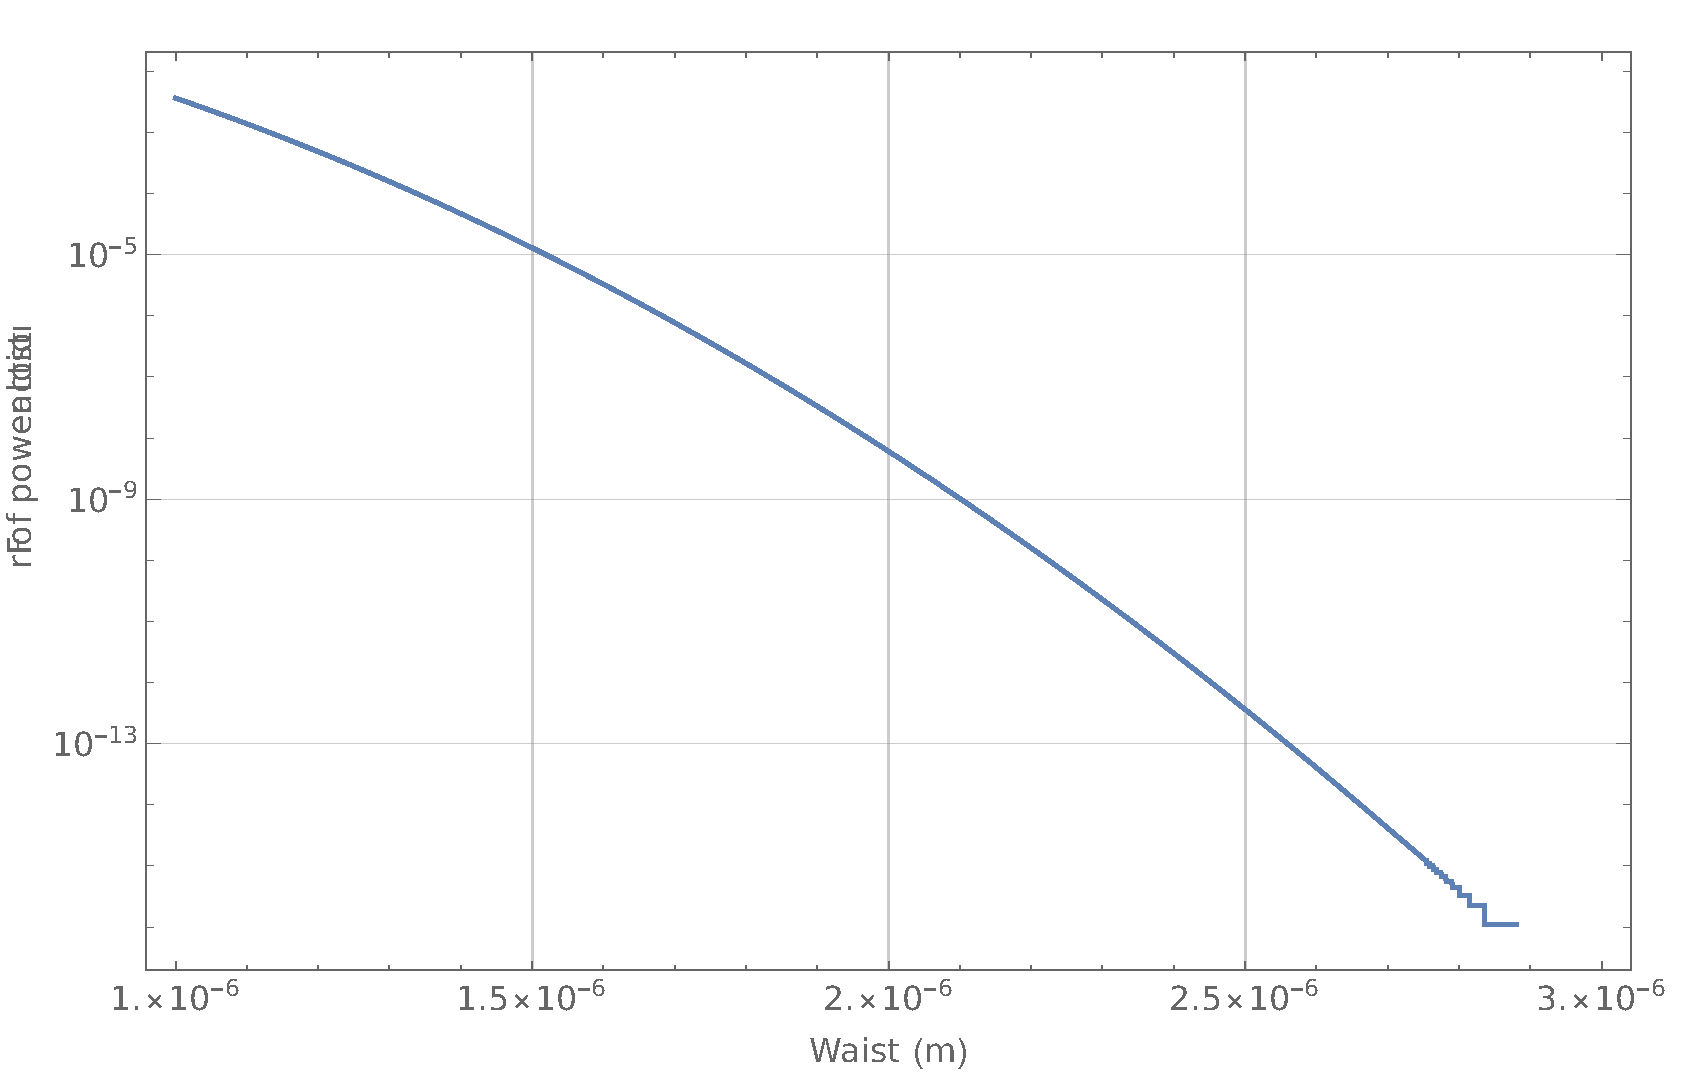
\includegraphics[width=.8\textwidth]{img/clipping2}
        \caption{Losses on the compensation electrodes as a function of the beam waist}
        \label{lossesplot}

\end{figure}

\begin{figure}
     \centering

     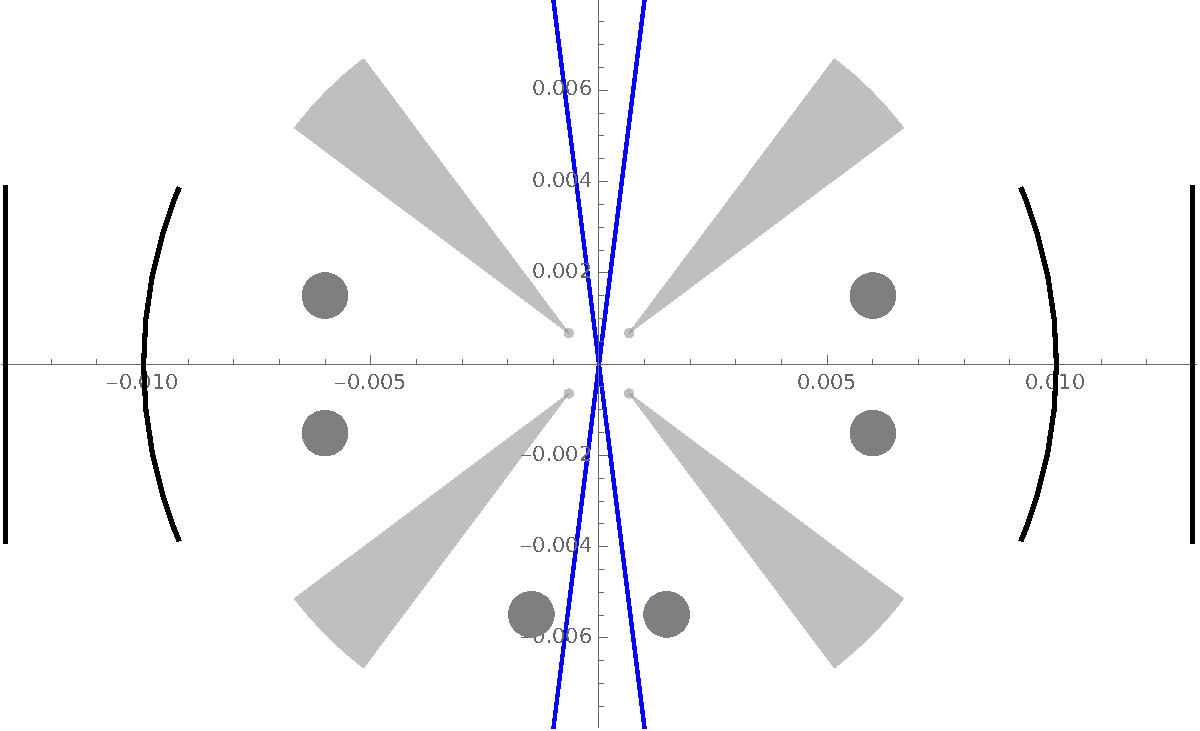
\includegraphics[width=.8\textwidth]{img/clipping}
     \caption{Top view of the trap and addressing beam. Grey circles are the compensation electrodes, blue is the radius $1/e^2$ of the beam, while the black arches representes the mirrors of the cavity.}
     \label{clippingtop}
     \end{figure}



\section{Physical implementation}
Once the simulations gave satisfactory results, a test setup was built. The idea of building first a test setup on a different optical table from the main experiment was to check if the system was working as intended, and asses its performance. Due to physical access problems, in the final system there is no space to place a beam profiler, or a polarimeter, and after the objective there is no access to the vacuum and the trap. While on another table everything could be checked and tested to make sure everything was working as expected. The results of the measurements obtained on this test setup are presented in the next chapter.\\
Afterwards, the real system was built. The building process was tricky, as the system is particularly sensitive to aberrations. Furthermore, there was not much room for alignment errors, since the trap and ion have to be hit perfectly. For this reason the alignment was essential. In order to make sure the addressing beam would hit the ion, a counter propagating red beam was send in the opposite direction, starting from the ion back to the objective and back to the addressing path. Since the lenses of the addressing are antireflecting coated for 393 nm, the reflection of the red beam was visible and it was possible to align every optical component. The photo of the final system is in figure \ref{photosetup}. Here the collimating lens is mounted on a 3D translation stage with Newport screws for fine tuning calibration of the focus position. Manual screw has been later replaced with remote controlled one always from Newport, model PZA12. An iris is also used to block the zeroth order beam from the AOD. Moreover, The AOD is placed on a rotational mount that allows to tilt it in two directions. One direction was used to find the Bragg angle to achieve maximum diffraction, and the other can be used to tilt the axis over which the AOD sweeps. This can be used to compensate for an ion string which is not exactly parallel to the AOD sweeping direction.

\begin{figure}[H]
\centering
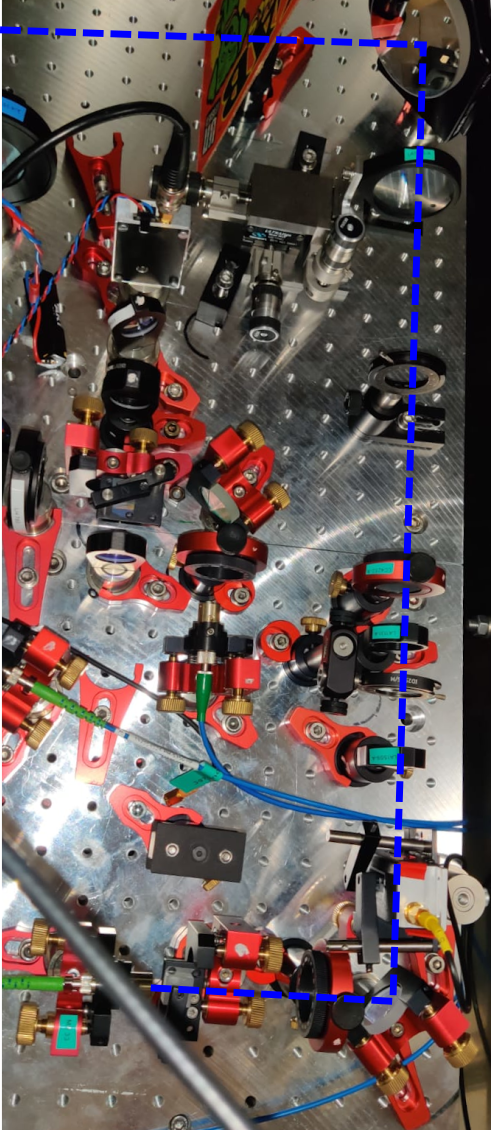
\includegraphics[scale = 1.3]{photosetupnice.png}
\caption{Photo of the final setup. The blue dashed line is the beam path starting from bottom left at the fiber collimator, all the way to the top where a mirror deflects the beam to send it to the beam splitter.}
\label{photosetup}
\end{figure}
